\documentclass[12pt]{article}

\usepackage{graphicx}
\graphicspath{ {../plots/} }
\usepackage{caption}
\usepackage{subfigure}

\title{Traffic Accidents Analysis}
\date{}

\begin{document}

\maketitle

% INTRODUCTION
% Introduce the project
% What is the data
% What is the goal
% How is the analysis structured?

% ANALYSIS

\section{Introduction}

The following is report is a deep look into traffic accident data provided by the British government for the year of 2019. There report is concerned with the two primary concerns of traffic accidents, the frequency at which they occur and their severity. Firstly, a general wide-ranging analysis was done to determine common trends in the data, followed by the testing of two distinct hypotheses. Finally, a probabilistic model was developed to predict both the temporal and spatial likelihoods of an accident, as well as its relative severity.

\section{Analysis}

\subsection{Data Cleaning}

The dataset as provided by GOV is fairly error free except for a few areas. twenty eight samples with missing coordinate data. However, all of these samples had local district information. Coordinate data for all towns and cities in the United Kingdom was scraped from the REF website using the Beautiful Soup package REF, and imputed according to the local district feature. 

A similar approach was taken to impute missing time values. In this case, the sunrise and sunset times for London were scraped from REF. According to the light conditions of the sample, the median time between sunrise and sunset on the day of the accident was imputed in the case of light, and the median time between sunset and sunrise in the case of darkness. The purpose of this was to ensure that imputed data does not contradict the obvious and empirically true covariance between the time of the day and light conditions.

\subsection{Primary Analysis}

Upon first inspection of the data, it was determined that there exist two primary SPIKES in accident frequency within the ranges 8am-10am, and then again from 3pm 7pm Figure \ref{time_of_day}. These are the times of commute, and so such increases are to be expected.

\begin{figure}[h]
\centering     %%% not \center
\subfigure[Accidents by time of day.]{\label{fig:a}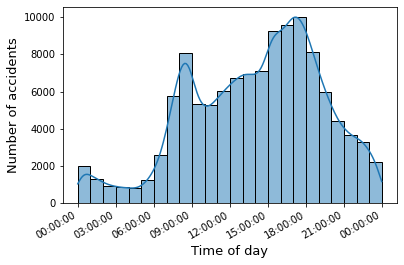
\includegraphics[width=0.45\textwidth]{time_of_day}}
\subfigure[Accidents by day of the week.]{\label{fig:b}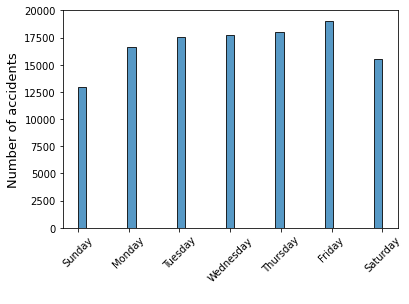
\includegraphics[width=0.45\textwidth]{day_of_week}}
\caption{Number of accidents.}
\end{figure}


\subsection{Hypothesis Testing}

A first hypothesis was tested to determine if there is a significant increase in traffic accidents surrounding football stadiums on the days of significant matches.

A test case was first carried out for the football match taking place at Old Trafford on Sunday 24th February 2019. Considering any accident within 5km of the stadium as being connected to the event, the accident count was compared against the number of accidents in this region every other Sunday during the year. On the day of the match, there were XNUM accidents in the region, 1.77 standard deviations above the mean. This was taken to be significant and worthy of further investigation.

Taking the premier league fixtures of 2019 REF, along with the coordinates of every premier league club stadium REF, the previous process was done iteratively for a total of 126 football matches during the year at 15 unique stadiums.

When summarised for every match, the z-score appears to be only 0.05 standard deviations from the average number of accidents. Although there is a significant difference in the number of accidents for different stadiums, on average the analysis implies that there is not a statistically significant rise in the number of accidents on the day of a football match compared to the typical same day of the week in the region.

The following table shows the summary statistics for premier league football matches. The second column shows the average number of accidents in the area of the stadium on days when there is a match, and the third column shows the average number of accidents on the same day of the week when there is not a match being played.

\begin{table}[!ht]
    \centering
    \begin{tabular}{|l|l|l|l|}
    \hline
        Stadium & Accidents 1 & Accidents 2 & z-score \\ \hline
        Anfield & 3.0 & 3.6 & -0.12 \\ \hline
        Cardiff City & 1.9 & 1.8 & 0.47 \\ \hline
        Craven Cottage & 16.1 & 16.4 & -0.08 \\ \hline
        Emirates & 21.6 & 21.5 & -0.01 \\ \hline
        Etihad & 3.8 & 5.2 & -0.56 \\ \hline
        Goodison Park & 3.3 & 3.5 & 0.01 \\ \hline
        King Power & 1.7 & 1.9 & 0.34 \\ \hline
        Molineux & 2.2 & 2.9 & -0.29 \\ \hline
        Old Trafford & 4.1 & 4.2 & -0.04 \\ \hline
        Selhurst Park & 14.2 & 11.7 & 0.63 \\ \hline
        Stamford Bridge & 17.1 & 19.9 & -0.47 \\ \hline
        Tottenham Hotspur & 16.4 & 16.5 & -0.0 \\ \hline
        Turf Moor & 0.0 & 1.0 & 0.0 \\ \hline
        Vicarage Road & 0.8 & 2.0 & -0.23 \\ \hline
        Wembley & 9.2 & 12.7 & -0.86 \\ \hline
    \end{tabular}
\end{table}

\section{Prediction}



\section{Conclusion}


% PREDICTIONS

% RECOMMENDATIONS

\end{document}